\documentclass[brief]{fub}  
\usepackage[utf8]{inputenc}   % ggf. das inputencoding aendern, z.B. "latin1"
\usepackage[english]{babel}
\usepackage{ansorge}         % hier steht der "basename" Ihrer .sty-Datei

\renewcommand{\adressvermerk}{} % ggf. Eintrag vornehmen

\renewcommand{\empfaengeradresse}{
  Boundary-Layer Meteorology \\ 
  To the editor\\
  Prof. William Anderson \\[0.5em]
  -- via E-Mail --
  
  
}

\begin{document}

\betreff{Submission of our manuscripts ``Wind veer and speed in turbulent Ekman flow Part I and II'' } 

\anrede{
  Dear Professor Anderson, 
}

We are pleased to submit two connected research papers on a topic of crucial importance for Boundary-Layer Meteorology,
namely the profiles on wind speed and direction in the lower part of the boundary layer.
%
The research papers are entitled
\begin{itemize}
\item[I] Wind veer and speed in turbulent Ekman flow Part I: Scaling Analysis and universal profile model
\item[II] Wind veer and speed in turbulent Ekman flow Part II: Extrapolation to Atmospheric Scale Separation
\end{itemize} 

%
This work tackles the problem of a consistent scaling framework across the different layers of the boundary layer,
including the viscous sub-layer, buffer layer, logarithmic layer, Ekman layer, and outer layer. Both papers 
are concerned with the study of idealized, stationary and truly neutral Ekman flow over a smooth surface. 
%
\par
%
In Part I, we approach the problem through DNS at unseen scale separation and domain size, we obtain high-quality data across all
these regimes that allow use to identify some robust features and scaling properties and yield valuable insight
on the scaling of stress, turbulent viscosity and the velocity profiles.
%
As we put a particular focus on the wind veer, the span-wise velocity component (which also accomplishes the Ekman transport)
is of central importance and we identify a novel mixed scaling of the component in the surface layer which allows us
to project the turning of the wind also within the lower part of the surface layer for arbitrary Reynolds number.
% 
\par
%
Part II builds upon these results using large-eddy simulation (LES). We beging with an a posteriori validation of the LES where
the DNS set-up is matched as exactly as possible in terms of Reynolds number and the z-nought parameter.
This yields valuable insight regarding the physical convergence of the LES to the DNS solution that serves as a reference here. 
%
Studies in typical, idealized amtmospheric-boundary-layer settings illustrate that the LES results are consistent with
the profile model that has been developed in part I and was calibrated using DNS data, provided the LES uses about 150 grid points to resolve the boundary layer.
%
The LES and the profile model developed are independent paradigms to study the velocity profile. Hence, the excellent agreement of LES and DNS data at low Reynolds number together with the agreement between LES and the profile model evaluated for geophysical Reynolds number suggests that both the LES and the profile model behave in a physical way for high Reynolds number. 
%
\par
%
We believe that our research makes a relevant contribution to the field.
%
The findings of this study, particularly of the surface layer similarity, are consistent and
complementary with atmospheric measurements.
%
The model developed in Part I is of practical relevance for applications in wind-power projection, numerical modelling
and can be used for a-priori testing of turbulence parameterizations in idealized settings. 
%
\par
%
We hope that the manuscript raises your interest and complies with the high standard of Boun\-da\-ry-Layer Meteorology and  would be delighted if the manuscript were considered for publication in the journal.

With Kind Regards, \vspace{-1em} 

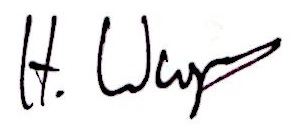
\includegraphics[height=1.3cm]{signature_hauke.jpg}~~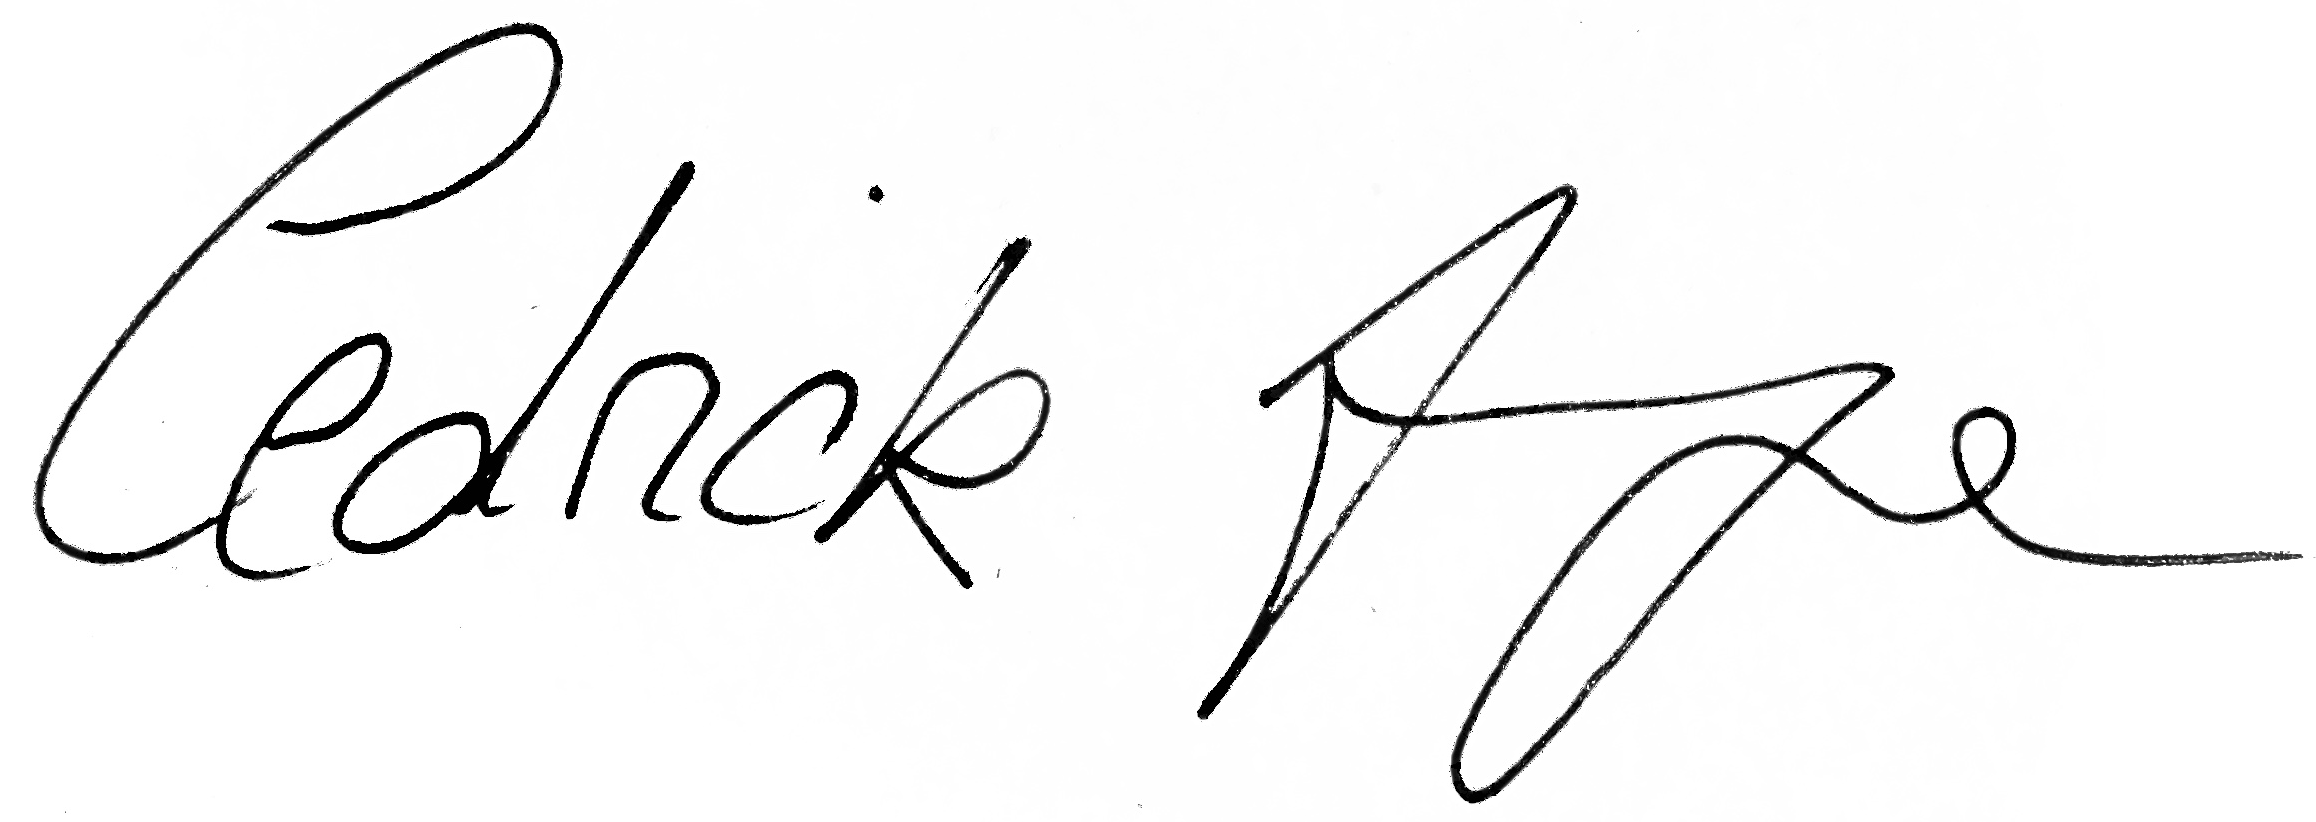
\includegraphics[height=1.5cm]{signature_transparent.png}\vspace{-2em}

Hauke Wurps \ \ \ \ \ \ \ \ \  Cedrick Ansorge

%\grussformelsigniert{With Kind Regards \vspace{-0.25em}}

\end{document}
